\documentclass[12pt]{article}

% TEMPLATE DEFAULT PACKAGES
\usepackage{amssymb,amsmath,amsfonts,eurosym,geometry,ulem,graphicx,color,setspace,sectsty,comment,natbib,pdflscape,array,adjustbox}

% ADDED PACKAGES FOR THIS MANUSCRIPT
\usepackage{palatino,newtxmath,multirow,titlesec,threeparttable,tabu,booktabs,titlesec,threeparttable,mathtools,bm,bbm,subcaption,pdflscape,tcolorbox,mathrsfs}
% endfloat,

\usepackage{afterpage}
\usepackage[hyphens]{url}
\usepackage[margin=1cm]{caption}

\usepackage[draft]{hyperref}
\newcommand{\tim}{$\,\times\,$}
% FIGURES & TABLES CAPTION STYLING
\captionsetup[figure]{labelfont={bf},name={Figure},labelsep=period}
\captionsetup[table]{labelfont={bf},name={Table},labelsep=period}

% SECTION TITLE SETTINGS
\titlelabel{\thetitle.\enskip}
\titleformat*{\section}{\large\bfseries}
\titleformat*{\subsection}{\normalsize\bfseries}

% COLUMN TYPES
\newcolumntype{L}[1]{>{\raggedright\let\newline\\\arraybackslash\hspace{0pt}}m{#1}}
\newcolumntype{C}{>{\centering\arraybackslash}p{5.2em}}
\newcolumntype{D}{>{\centering\arraybackslash}p{5em}}
\newcolumntype{R}[1]{>{\raggedleft\let\newline\\\arraybackslash\hspace{0pt}}m{#1}}


% MARGINS AND SPACING
\normalem
\geometry{left=1.1in,right=1.1in,top=1.0in,bottom=1.0in}
\setlength{\parskip}{2.5pt}

% SPECIAL CELL 
\newcommand{\specialcell}[2][c]{%
	\begin{tabular}[#1]{@{}l@{}}#2\end{tabular}}

% NO INDENT ON FOOTNOTES
\usepackage[hang,flushmargin]{footmisc}

\begin{document}

\begin{titlepage} 
\title{{Paying bills}\thanks{We are grateful to Andrew Foster}}
\author{\\[3em]
  William Violette\thanks{Federal Trade Commission, Washington, DC. E-mail: william.j.violette@gmail.com} \\
 \\ 
  }
\vspace{30mm}
\date{\vspace{5mm}This Version: \today}
\maketitle
\begin{abstract}

	paying bills

 %\\

%\vspace{0in}\\
%\textbf{Keywords:} traffic externalities; street livability; urban policy; housing market.\\
%\vspace{0in}\\
%\textbf{JEL Codes:} O18; H4; R2; R4.\\
\bigskip
\end{abstract}
\setcounter{page}{0}
\thispagestyle{empty}
\end{titlepage}
\pagebreak \newpage

\spacing{1}


\section{Pitch}

This paper looks at whether utilities in developing countries provide an important source of credit to households by letting them not pay their bill?  And how do these benefits compare to the costs of delinquency?

Motivation : (1) around the world, there are restrictions on when utilities can disconnect people (health, low-income, elderly), motivated by providing a sense of insurance;  (2) Also, in developing countries, pre-paid metering where utilities essentially put fancy meters that only distribute water when people pay first.  these shut off any credit channel but eliminate delinquency

Context : In Manila, water bills make up about 3\% of income on average, jumps to 5 to 10\% for low-income folks.  I have data from a large water provider serving half the city of Manila.  On average, people make a payment in three out of four months and are about a month behind in payments.  For example, if you don't pay for three months, that's like taking a three-month loan of around 9\% of your income.  

People might be paying infrequently because they are credit-constrained and consumption smoothing; or it might just be a pain to pay their bills so they just avoid the hassle by paying infrequently (and they have plenty of other opportunities to smooth).  

I use disconnection threats to better isolate the role of credit constraints.  Workers will occasionally visit delinquent customers and say if you don't pay your bill soon (within 12 days on average), we'll disconnect you.  Only 23\% of people say that's ``enough time'' to pay the bill.  After the threats, payments spike to double the average bill, delinquency drops to zero, and consumption drops by around 25\%.  If it were simply a hassle, people would pay their bill and consumption wouldn't change (they could get easy credit from other places and pay the bill); but if they are credit constrained, they have to deviate from consumption smoothing to make the payments.  The next step is to use theory to see what this decrease in consumption implies about the short-term interest rate that households face.


\section{Introduction}

%% disconnection 

% https://liheapch.acf.hhs.gov/Disconnect/disconnect.htm
\subsection{Question} 
Are utilities providing an important source of credit to households by letting them not pay their bill?

\subsection{Motivation}
\begin{itemize}
\item Disconnection policies as insurance (in the US) 
	\begin{itemize}
		\item weather, health, low-income
		\item mandate that utilities amortize arrears
		\item Utilities even tolerate greater non-payment
	\end{itemize}
\item At the same time, pre-paid metering is growing like crazy in the developing world (Sources)
\end{itemize}

\subsection{Descriptives}
% How much credit could households get from their water bill?
\begin{itemize}
\item Avg Income: 22,000 PhP (488 USD)   [ Bill 3\% ]
\item Avg Savings: 4,300 PhP (96 USD) 
\item 20\% Income: 8,300 PhP (184 USD)  [ Bill 7.6\% ]
\item 20\% Savings: 330 PhP (7 USD)  
\item Avg Bill: 630 PhP (14 USD)
\item Make payments 75\% of months
\item Avg delinquency: 30 days
\item Avg Payment Amount: 830 PhP (18 USD)
\end{itemize}

But : might just be inconvenient to pay every month (but its really easy to pay bills in this context)

How can I ballpark this against the consumption smoothing literature?

\subsection{Approach}

Disconnection : Don't pay bill; come and threaten disconnection
\begin{itemize}
\item avg days to pay : 12 days (only 23\% say that's enough time)
\item if you (agree to?) pay, you are reconnected after 2 days
\item 30\% of connections are threatened with disconnection
\item (small percent actually disconnect)
\item Pay (+1) 800 PhP (+2) 300 PhP = total 1100 PhP (24 USD) [ about two water bills on average ]
\item Consumption drops by about 20\% for two months (there is a pre-trend which can be interpreted as positive demand shocks)
\end{itemize}

\noindent Theory :
\begin{itemize}
\item suddenly this source of credit is cut off (loan with uncertain payback date)
\item concave utility predicts that households would want to smooth consumption (could get another loan, then fund consumption in that period)
\item 
\end{itemize}


\section{Data}

To measure water consumption and payments, I partnered with a large water provider in Manila who shared administrative data on over 1.5 million water connections.  These data include water consumption and payment data as well as disconnection status. 

Describe notice of disconnection in more detail here???

used to measure water consumption and payment data comes from monthly administrative data from a large water provider in Metro Manila


The 2015 Family Income and Expenditure Survey provides household income measures, which help to calibrate the structural model.  

STICK WITH ONE HOUSEHOLD PER METER IN THIS PAPER!  EXPLAIN THIS IN THE DATA SECTION!

\section{Credit through Unpaid Water Bills in Manila}

\begin{table}
\centering
\caption{Descriptives}\label{table:descriptives}
 Usage (m3)  & 26.2  & 17.5  & 0.0  & 15.0  & 33.0  & 200.0  \\ 
 Bill  & 761  & 1,124  & -4,640  & 287  & 920  & 78,409  \\ 
 Unpaid Balance  & 2,416  & 5,070  & -4,995  & 261  & 2,346  & 79,904  \\ 
 Share of Months with Payment  & 0.60  & 0.49  & 0.00  & 0.00  & 1.00  & 1.00  \\ 
 Payment Size  & 734  & 1,308  & -25,675  & 0  & 1,000  & 61,298  \\ 
 Days Delinquent  & 84.9  & 155.4  & 0.0  & 0.0  & 91.0  & 720.0  \\ 
 Delinquency Visits per HH  & 1.322  & 0.606  & 1.000  & 1.000  & 2.000  & 6.000  \\ 
Months Disconnected  & 0.031  & 0.174  & 0.000  & 0.000  & 0.000  & 1.000  \\ 

\end{table}

At the end of each month, the water company sends meter readers who record monthly consumption for each connection and then use a mobile device to print and deliver the bill to the household in person.\footnote{The company upgraded in the first year of the sample.  Previously, the company mailed the bill to each household at the end of the month.}  The household is then expected to pay the bill by the end of the month.  Households have many options to pay their bills with 79\unskip\% using small payment centers (mall kiosks, gas stations, convenient stores, etc.), 9.4\unskip\% paying at local water company offices, 3\unskip\% paying over phone, online, or via ATM kiosks, and 0\unskip.2\unskip\% paying the meter readers in person.\footnote{Figures are tabulated from the connection survey.}  

Despite encouragement from the company and easy payment mechanisms, households rarely pay their bills on time.  Table~\ref{table:descriptives} provides summary statistics on the usage, billing, and payment patterns of households.  On average, households are 97.0days behind in their payments.  Households also make large, infrequent payments.  While the average bill is 587.8PhP per month, monthly payments average 1,049.7PhP and households make payments in only 61\unskip\% of months.  These payment patterns amount to an average outstanding balance of 1,387.3 per month.  

Since the government regulator also prohibits the water company from charging any interest on outstanding balances, unpaid water bills can provide a reliable source of low-cost credit to households.  Given an average monthly income of 31,910PhP and savings rate of 5,730PhP, unpaid water bills reach an average of 4.3\unskip\% of income and 28.7\unskip\% of savings.

After a connection has remained unpaid for a minimum of 60 days, the government regulator allows the water company to issue a written statement to the connection owner, notifying the owner that their water will be disconnected in 7 days if their outstanding balances remain unpaid.  In practice, the water company often tolerates delinquency well over 60 days, which is consistent with (1) costs of sending and following up on notifications and (2) household demand for credit from the water company.  Households receive notice in 0.66\unskip\% of months.  This rate increases to 1.75\unskip\% for households with at least 60 days of delinquency.  Figure~\ref{figure:dc_hazard} graphs the probability of receiving a delinquency notice conditional on the level of delinquency for each account.  The water company appears to carefully follow government regulations preventing any disconnection for delinquency below 60 days.  Once households reach 61 days of delinquency, they face some probability of receiving a notice, which triples moving above 90 days unpaid balance.  Conditional on having greater than 90 days of delinquency 


\begin{figure}
\centering
\caption{Probability of Notice Conditional on Days Delinquent}\label{figure:dc_hazard}
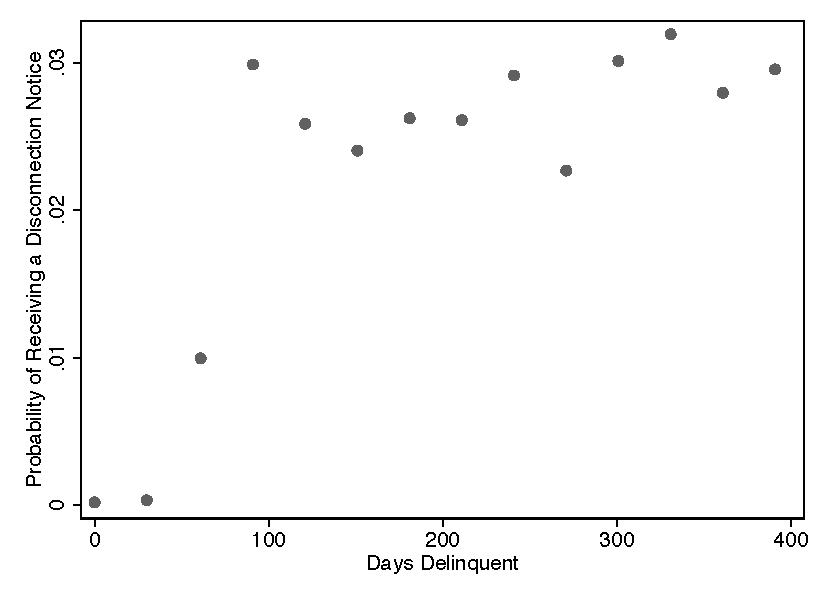
\includegraphics[scale=.7]{tables/dc_hazard_full.pdf}
\end{figure}



% Appendix on notice!  ( need to get water company confirmation )

%  In practice, the water company tolerates 108.1days of delinquency on average before issuing a notice.  The level of delinquency tolerated before issuing notices also appears uncorrelated with (list measures/demographics...).  ( SHOW REGRESSION IN APPENDIX )  

Upon receiving a notice of disconnection, connection owners then negotiate for time to pay their outstanding balances.  In 96\unskip\% of notices, owners are agree to pay within 30 days, making an average grace period of 13days according to the water connection survey.  25\unskip\% of connections report having ``enough time'' to make their payments.  

%The administrative data indicate that 72.5\unskip\% resolve their outstanding balances following a notice.

Disconnection typically involves workers from the water company placing a metal lock on the water meter stopping the flow.  Once disconnected, connection owners are charged a small, one-time fee of 200 PhP to restore their water service on top of settling any outstanding balances.  The water company is then required to restore service within 48 hours of receiving full payment for reconnection.





\begin{itemize}
	\item No notice: great access to credit, or just not enough time to observe them hitting a
	\item Average notice rate!?!

\end{itemize}




%\footnote{To account for potential mismeasurement in the administrative data, this measure allows connection owners to resolve their outstanding balances within 60 days of receiving notice.}

%In practice, .\unskip\% of owners report receiving advanced notice.  







\section{Model Primitives}

% https://www.cgdev.org/blog/compartamos-context


\cite{karlan2009expanding} find money lenders regularly charge at least 20\% per month for credit.  \cite{gine2014group} offer small monthly loans of 1,000 PhP at 2.5\% monthly interest.

\cite{andreoni2012estimating} estimate rates between 25\% and 35\% in an experimental setting and confirm exponential discounting.  \cite{laibson2007estimating} use a similar consumption-savings structural approach and recover a discount rate of around 15\%.  \cite{gourinchas2002consumption} use a similar structural approach finding a lower discount rate of around 5\%.



%%% Karlan and Zinman

% Informal credit markets
% and serial borrowing from moneylenders charging 20% per month or more is common (e.g., more than
% 30% of our sample reported borrowing from moneylenders during the past year). Trade credit is quite
% uncommon. There are several microlenders operating in Metro Manila, but most MFIs operate on a
% small scale (as noted above) and charge high rates (see below).


\section{Results}

\begin{table}
\centering
\caption{Estimates}\label{table:estimates}
\begin{tabular}{lcc}
& Estimate & Standard Error \\
Interest Rate &0.046&0.00\\
Income Variance &0.300&0.00\\
Water Preference &0.020&0.00\\
\end{tabular} 

\end{table}

\begin{table}
\centering
\caption{Fit}\label{table:fit}
\begin{tabular}{lcc}
& Data & Estimated \\
Mean Usage (m3) &24.9&25.5\\
SD Usage &11.1&2.2\\
Mean Water Debt (PhP) &1232&1222\\
SD Water Debt (PhP) &1281&1821\\
Corr. Usage and Water Debt &0.34&-0.01\\
Mean Usage Pre-Collect (m3) &26.2&25.2\\
Mean Usage Post-Collect &23.4&22.7\\
Diff. (Pre-Post) (m3) &2.8&2.5\\
\end{tabular} 

\end{table}

\begin{figure}
\centering
\caption{Simulated Months}\label{figure:deaton}
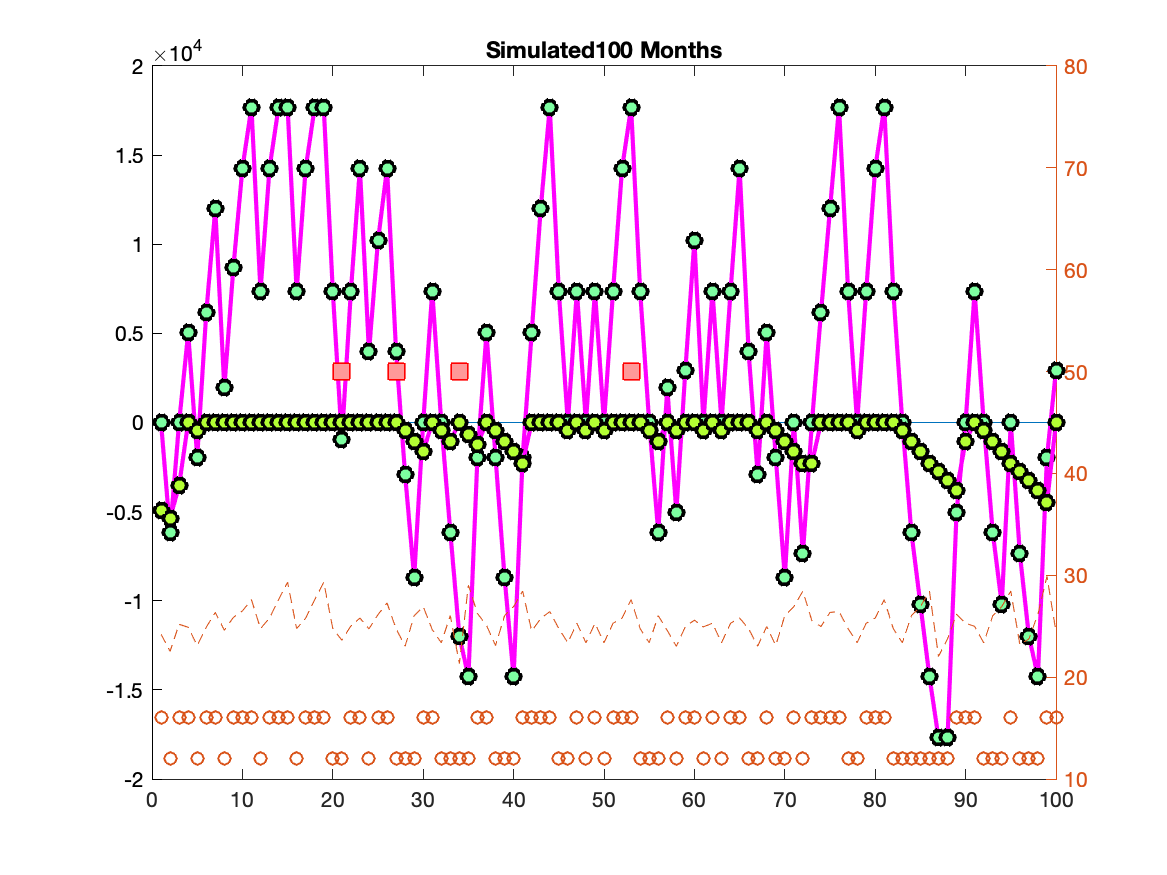
\includegraphics[scale=.5]{tables/deaton.png}
\end{figure}

\begin{table}
\centering
\caption{Counterfactuals}\label{table:counter}
\begin{tabular}{lccc}
& Current & No Water Credit & No Water Credit and \\
&         &                  & Revenue Neutral \\
Water Credit Interest Rate &0.0&1.0&1.0\\
Mean Usage (m3) &25.5&24.2&26.1\\
Compensating Variation  & &51.6&1.4\\
Delinquency Savings  &20.8&20.8&0.0\\
Price Intercept  &16.3&16.3&13.5\\
\end{tabular} 

\end{table}


\nocite{*}
\singlespacing
\setlength{\bibsep}{7pt}
\bibliographystyle{abbrvnat}
\bibliography{ref}



\end{document}


